\documentclass[journal]{IEEEtran}

%%%%%%%%%%%%%%%%%%%%%%%%%%%%%%%%%%%%%%%%%%%%%%%%%%%%%%%%%%%%%%%%%%%%%%%%%%%%%%%%
%
% Package
%
%%%%%%%%%%%%%%%%%%%%%%%%%%%%%%%%%%%%%%%%%%%%%%%%%%%%%%%%%%%%%%%%%%%%%%%%%%%%%%%%
\usepackage{ifpdf}
\ifCLASSINFOpdf
  \usepackage[pdftex]{graphicx}
  % declare the path(s) where your graphic files are
  % \graphicspath{{../pdf/}{../jpeg/}}
  % and their extensions so you won't have to specify these with
  % every instance of \includegraphics
  \DeclareGraphicsExtensions{.pdf,.jpeg,.png}
\else
  % or other class option (dvipsone, dvipdf, if not using dvips). graphicx
  % will default to the driver specified in the system graphics.cfg if no
  % driver is specified.
  \usepackage[dvips]{graphicx}
  % declare the path(s) where your graphic files are
  % \graphicspath{{../eps/}}
  % and their extensions so you won't have to specify these with
  % every instance of \includegraphics
  \DeclareGraphicsExtensions{.eps}
\fi

\usepackage[utf8]{inputenc}
\usepackage[T1]{fontenc}
\usepackage[french, english]{babel}
\usepackage{cite}
\usepackage{caption}
\usepackage{amsmath,amsfonts,amssymb}
\usepackage{subcaption}
\usepackage{array}
\usepackage{color}
\usepackage{float}
\usepackage{multicol}
\usepackage[]{algorithm2e}
\usepackage{hyperref}
\usepackage{fancyhdr}
%
% correct bad hyphenation here
\hyphenation{op-tical net-works semi-conduc-tor}

\DeclareMathOperator*{\argmin}{arg\,min}
\DeclareMathOperator*{\argmax}{arg\,max}

\begin{document}

\begin{IEEEbiography}[{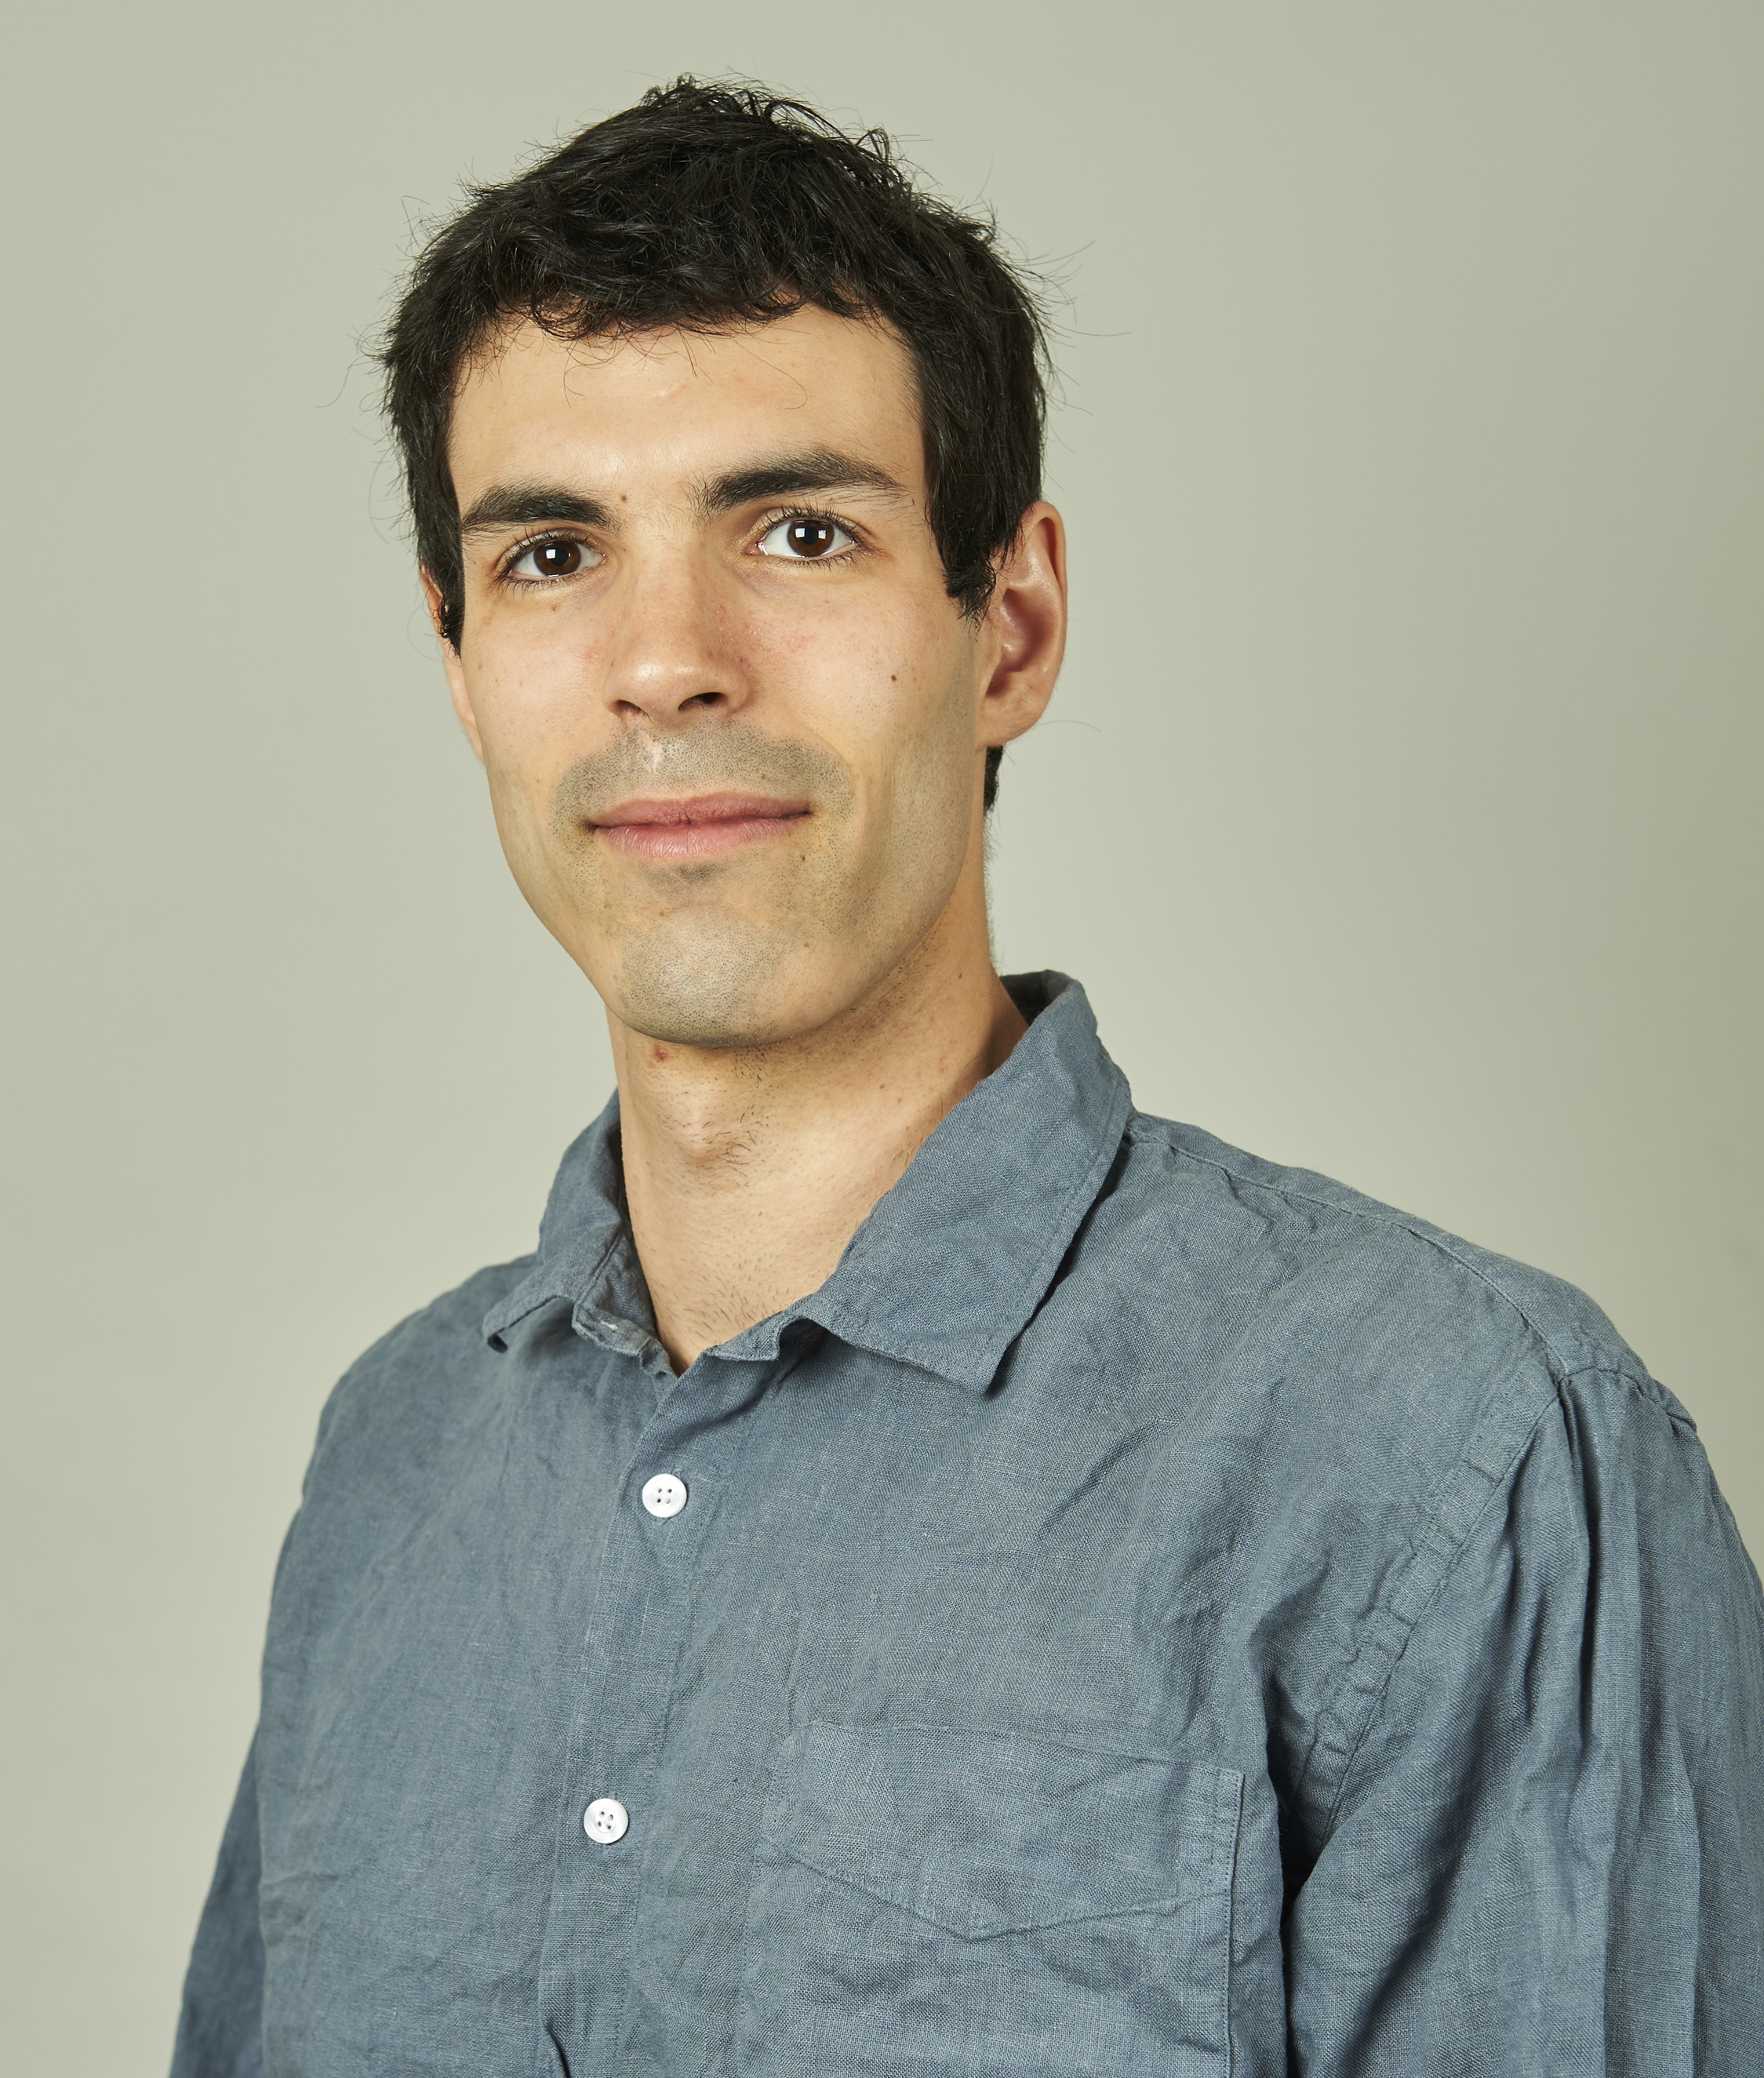
\includegraphics[width=1in,height=1.25in,clip,keepaspectratio]{Nicolas_Gensollen.jpg}}]%
{Gensollen Nicolas}
was born in Paris in 1989. He received the telecommunication engineer degree from Telecom SudParis in 2012 with a specialization in networking. He is currently a PhD student at the Institut Mines-T\'el\'ecom, T\'el\'ecom SudParis, France. His current research interests are mainly on smart grid, complex systems, and agent based modeling. Other research interests include dynamics and control in networks and game theory. 
\end{IEEEbiography}



\begin{IEEEbiography}[{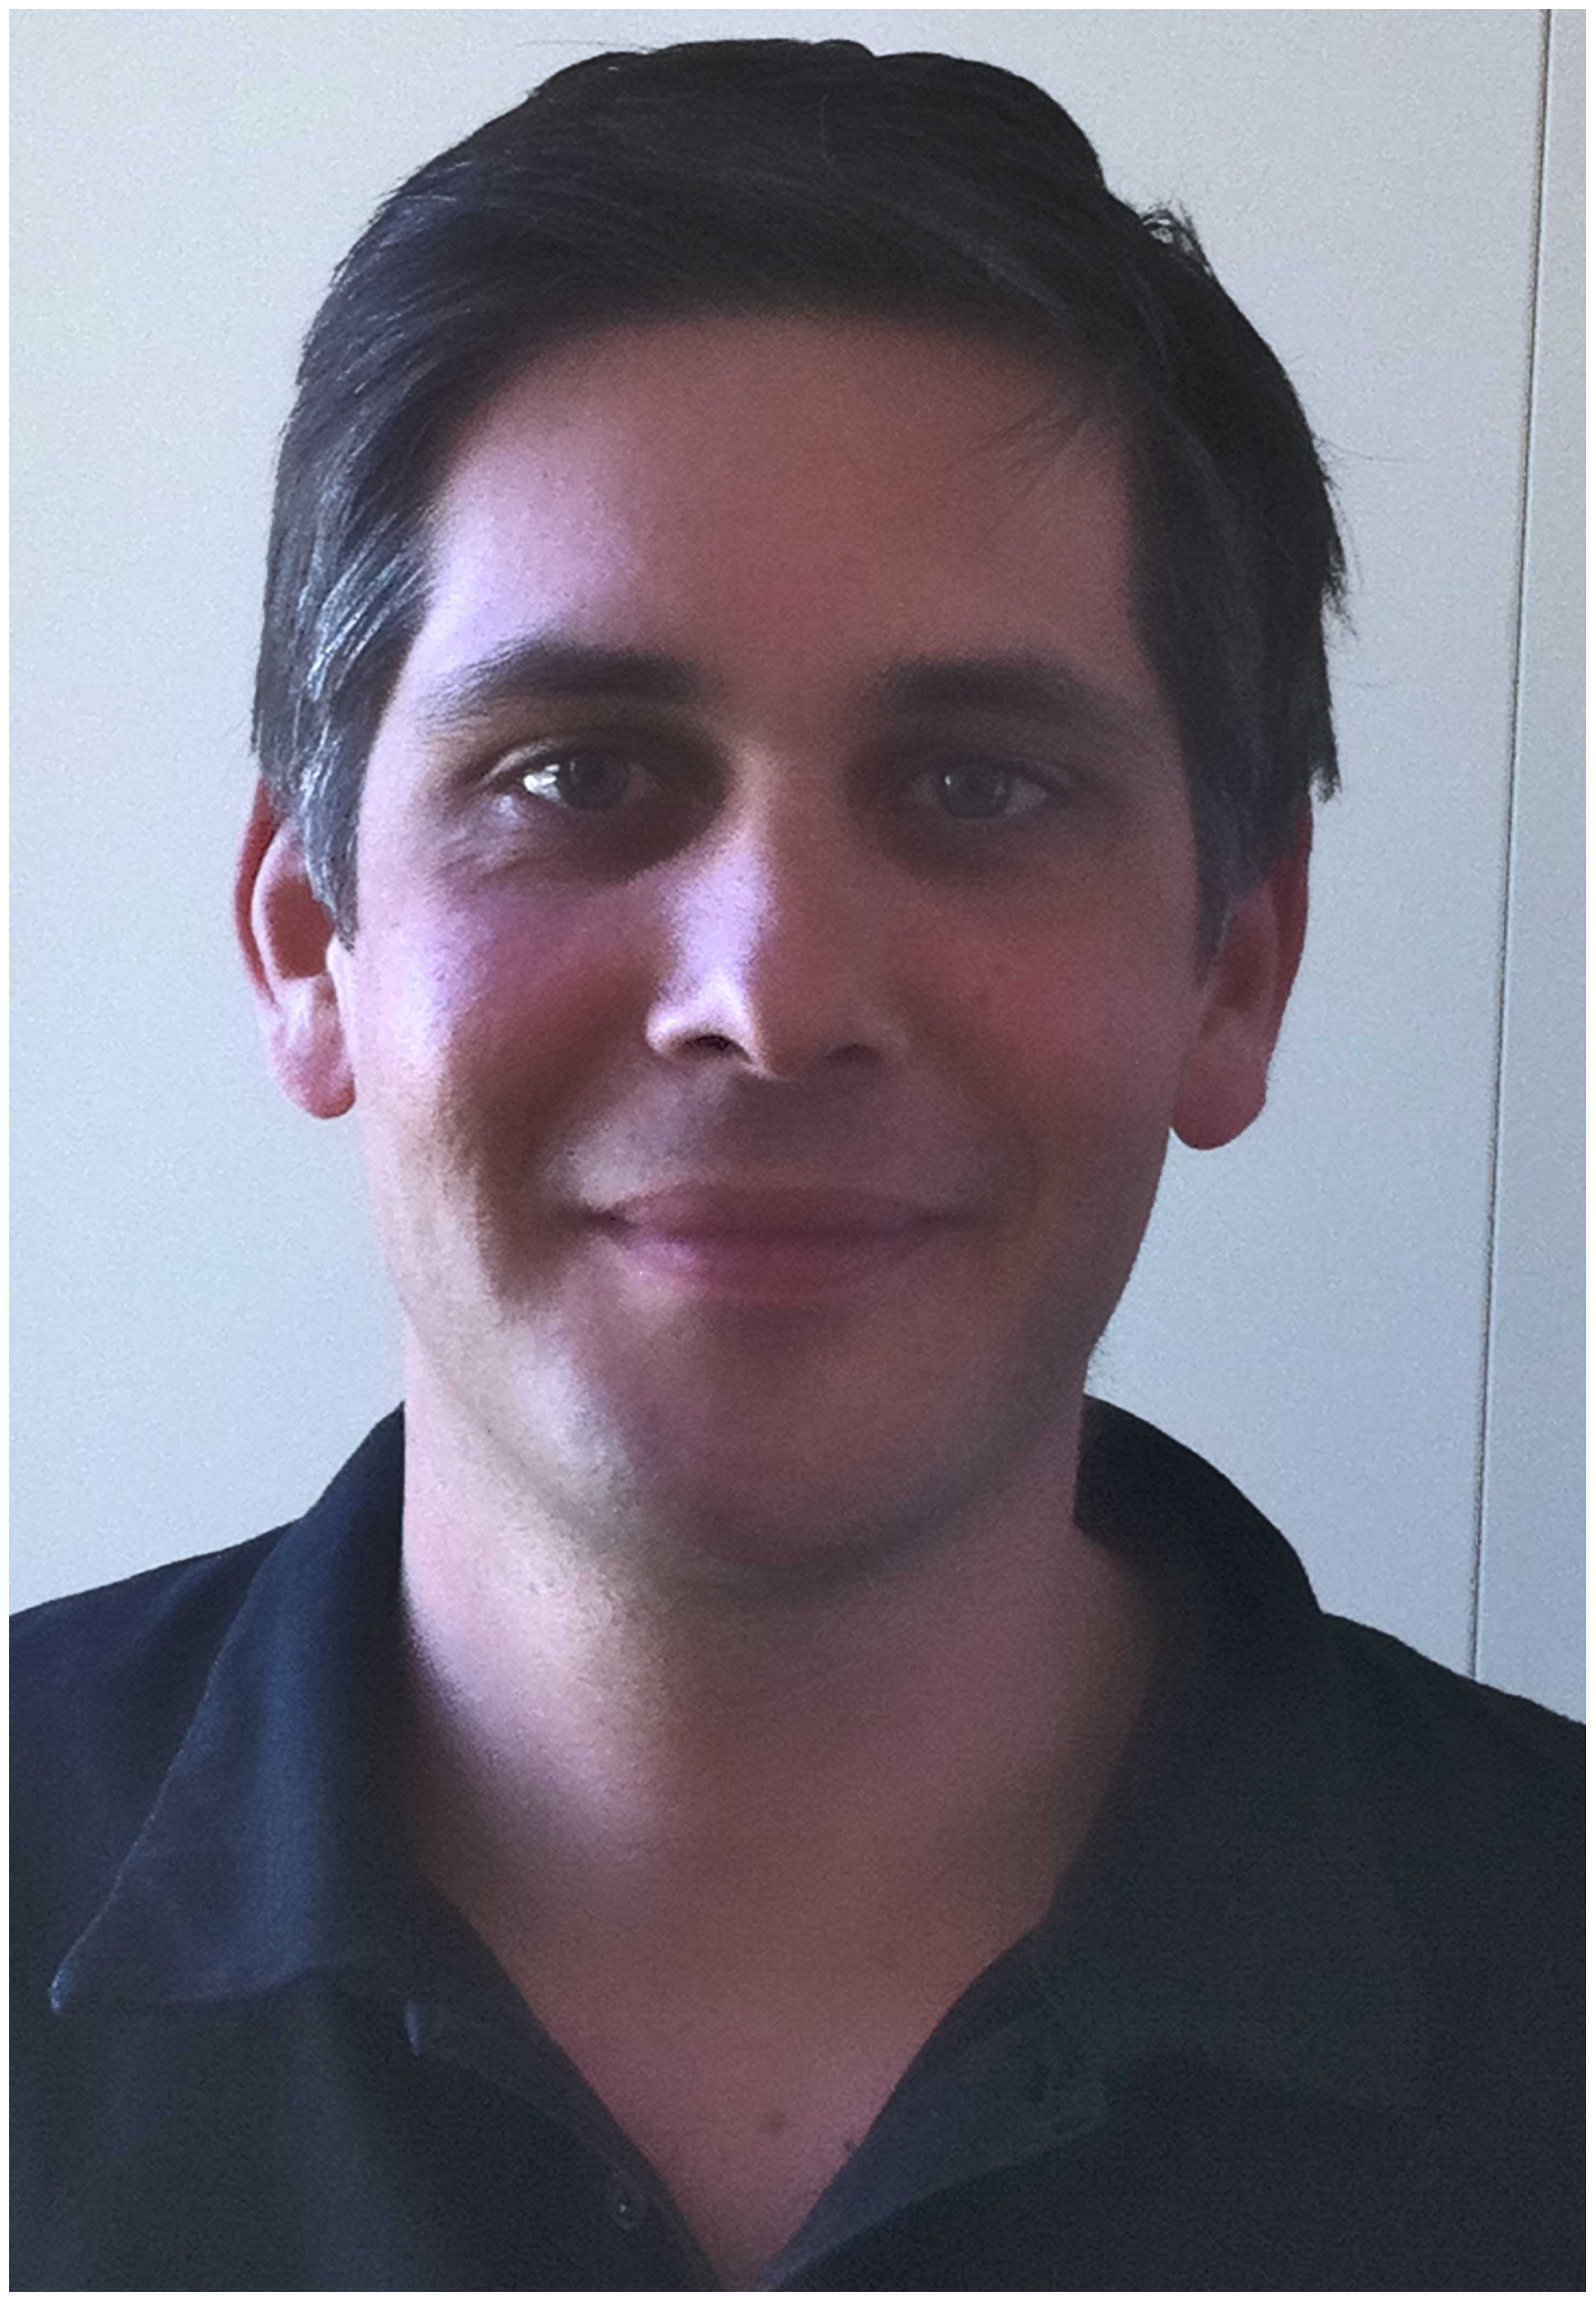
\includegraphics[width=1in,height=1.25in,clip,keepaspectratio]{Bio_Vincent.eps}}]%
{Gauthier Vincent}
was born in Paris in 1978. He received the B.S. in electrical engineering from University de Bretagne Occidentale in 2002 and M.S. degrees the Ph.D. degree in computer science and computer networks from University of Paris 6 in 2003 and 2006, respectively. He was a Guest Researcher at National Institute of Standards and Technology, MA, United States between 2006 and 2008. He joined the faculty of Telecom SudParis, and the lab CNRS SAMOVAR (UMR 5157), Evry, France, in 2008, where he is currently an Associate Professor of the Department of Computer Network. His current research interests are primarily on computer networks, self-organization and complex systems. His other research interests include mobility modeling, performance analysis, and queuing theory, sensor networks, ad-hoc networks, cross-layer design.
\end{IEEEbiography}



\begin{IEEEbiography}[{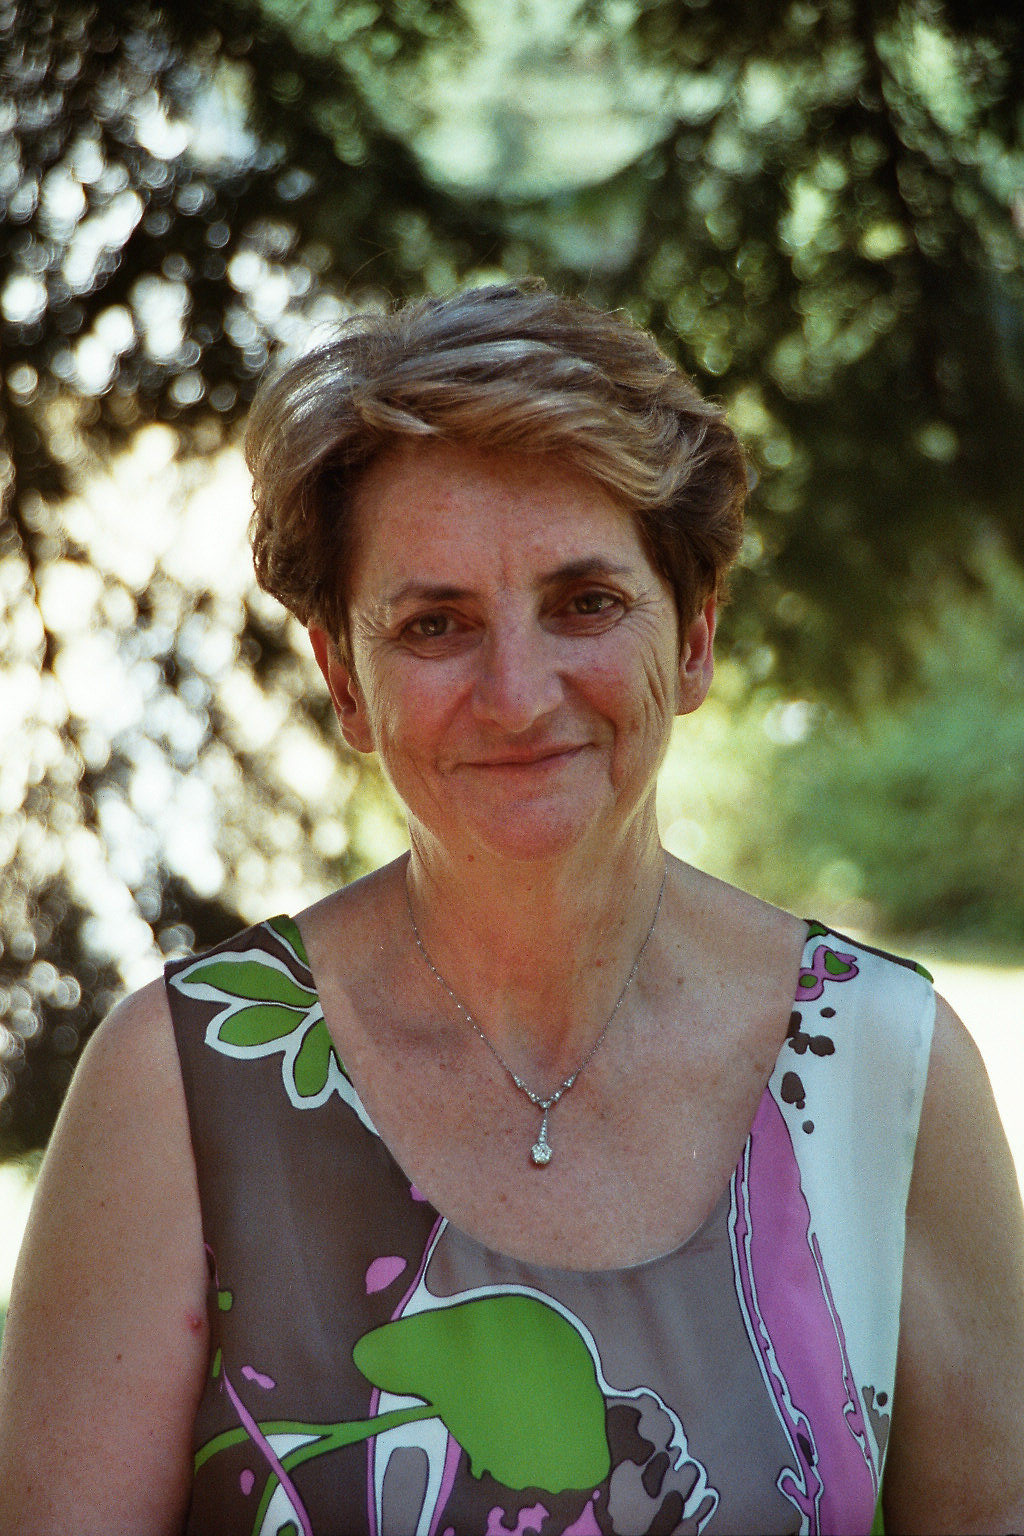
\includegraphics[width=1in,height=1.25in,clip,keepaspectratio]{Monique_Becker.jpg}}]%
{Becker Monique}
who studied Maths at ENSJF was a researcher at CNRS in Paris VI University from 1968 to 1987, and then a Professor at Telecom SudParis, till 2015. She is now an Emeritus Professor in Institut Mines-Telecom.
Her PhD concerned “validity of simulations” and her research work concerns mostly Performance Evaluation and Modelling of Networks and Distributed Systems. She designed aggregation methods for performance evaluation. She wrote a book, with her PhD students on Network simulations. 
She was the Director of the CNRS UMR5157: Samovar, since its starting and during 10 years.
She was the director of about 50 PhD students.
She started in 2001 a Master course taught in English: “Computer and Communication Networks” in Telecom SudParis. This Master is now taught in Paris Saclay University.
She was an expert for NSF, for NSERC (Canada) and for the European Commission.
She mostly collaborates with research groups in USA, in Austria, in Singapore and in India.

\end{IEEEbiography}



\begin{IEEEbiography}[{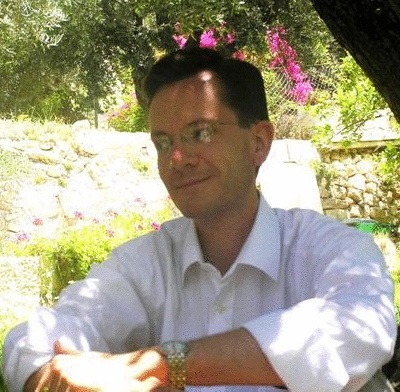
\includegraphics[width=1in,height=1.25in,clip,keepaspectratio]{michel_marot.jpg}}]%
{Marot Michel}
was born in Paris in 1973. He received the Ph.D. and habilitation degrees in computer networks from University of Paris 6 in 2001 and 2010. He is a professor in the Telecommunication Networks and services department at the Institut Mines-T\'el\'ecom, T\'el\'ecom SudParis, France. His current research interests are mainly on network performance and self-organization in wireless networks, ad-hoc and sensor networks, vehicular networks, context aware adaptation. His other research interests include mobility modeling, complex systems, and queuing theory and more generally performance of distributed systems.
\end{IEEEbiography}

\end{document}